\section{Physikalische Grundlagen}

\subsection{Funktionsweise eines Lasers}


Der Laser stellt eines der wichtigsten Werkzeuge der Experimentalphysik dar. Es gibt viele
verschiedene Arten von Lasern, die grundsätzliche Funktionsweise ist jedoch immer ähnlich. Man
benötigt zunächst ein aktives Medium, in dem optische Übergänge stattfinden, die zur Emission von
Photonen führen. Außerdem benötigt man eine optische Pumpe, die eine Besetzungsinversion im Medium
erzeugt, wodurch sich mehr Atome im Zustand höherer Energie befinden. Dazu benötigt man mindestens
drei Zustände: Einen Grundzustand, von dem aus die Elektronen in einen ersten angeregten Zustand
gepumpt werden, welcher mit möglichst kurzer Lebensdauer in einen weiteren angeregten Zustand etwas
niedriger Energie fällt, der eine möglichst lange Lebensdauer besitzt. Dies verhindert, dass die
Photonen des Laserlichts direkt wieder absorbiert werden und Atome im niedrigen Zustand
anheben. Zusätzlich benötigt man einen Resonator, der Photonen mit einer bestimmten Energie und
Impuls in den Laser zurückkoppelt. Diese Photonen regen dann Atome dazu an, in den niedrigeren
Zustand zu fallen und dabei ein Photon mit gleicher Energie und Impuls zu emittieren. Das führt zu
dem gewollten monochromatischen und kohärenten Licht.
Wenn mehrere verschiedene Übergänge zur Verfügung stehen, wird die Wellenlänge des Lasers durch die
minimalsten Verluste sowie die Wirkungsquerschnitte der Übergänge bestimmt. Die Verluste sind
hierbei vor allem vom Resonator beeinflusst, zum Beispiel über die Reflektivität der Spiegel.



\subsection{Stabilitätskriterium des Resonators}


Ein Resonator ist stabil, wenn ein Strahl auch nach beliebig vielen Reflexionen den Resonator nicht
verlässt.
Mit Hilfe von Matrizenoptik lässt sich dafür das Stabilitätskriterium eines Resonators
ableiten:

\begin{equation}
0\leq g_1 \cdot g_2 \leq 1
\end{equation}

wobei $g_1=(1-\frac{L}{R_1})$ und $g_2=(1-\frac{L}{R_2})$ mit den Krümmungsradien der Spiegel
$R_{1/2}$ und dem Abstand der Spiegel L. In diesem Versuch verwenden wir hauptsächlich einen
hemisphärischen Resonator mit einem Spiegel mit einem Krümmungsradius von 100\,mm, für die
Frequenzverdopplung wird jedoch ein sphärischer Resonator benötigt mit einem zweiten Spiegel mit
einem Krümmungsradius von 150\,mm.
In Abb.~\ref{img:stabkrit} sind die Verläufe von $g_1 \cdot g_2$ als Funktion des Abstands der
Spiegel dargestellt. Daraus ergibt sich für den hemisphärischen Resonator ein stabiler Zustand für
einen Abstand bis 100\,mm und für den sphärischen Resonator zusätzlich von 150\,mm bis 250\,mm.

\begin{figure}[H]
\begin{center}
  \includegraphics[width=.7\textwidth]{Stabkrit1.pdf}
  \caption{Darstellung des Stabilitätskriteriums für unsere verwendeten Laserresonatoren als
  Funktion des Abstands der Spiegel. Für $g_1\cdot g_2$ zwischen 0 und 1 ist der Resonator stabil.}
  \label{img:stabkrit}
\end{center}
\end{figure}


\subsection{Eigenschaften des Pr:YLF-Lasers}


In diesem Versuch verwenden wir als aktives Lasermedium das Praseodym (Pr$^{3+}$), welches in
einen Yttrium- Lithium- Fluorid (YLF) Kristall eingebettet ist. Das Energieschema ist in Abb.~\ref{img:Termschema} zu sehen und entspricht einem vier Niveau System. 
Vom Grundzustand $^3$H$_4$ aus wird mit einer Wellenlänge von 444\,nm in den ersten angeregten Zustand $^3$P$_2$ gepumpt. Dieser zerfällt mit einer kurzen Lebensdauer ohne Aussendung von Strahlung in die Zustände $^3$P$_1$ und $^3$P$_0$ welche eine deutlich längere Lebensdauer besitzen und als zweite angeregte Zustände die Ausgangszustände des Laserlichts sind. Von dort findet nun stimulierte Emission hauptsächlich in die Zustände $^{3}$F$_{4,3,2}$ und $^3$H$_{6,5}$ statt. Diese Zustände zerfallen schlussendlich wiederum mit einer kurzen Lebensdauer ohne Aussendung von Strahlung in den Anfangszustand $^3$H$_4$.

Die Vorteile der Verwendung von Praseodym liegen hauptsächlich in der Vielzahl unterschiedlicher Laserlinien und der Tatsache, dass diese im sichtbaren Spektralbereich liegen. Der sehr weit verbreitete Nd:YAG Festkörperlaser emittiert im Vergleich dazu lediglich im infraroten Bereich hauptsächlich bei 1064\,nm. Dadurch ist auch das erzeugen von UV-Strahlung deutlich einfacher, da hier die Frequenz lediglich verdoppelt werden muss anstatt verdreifacht wie beim Nd:YAG Laser.
Außerdem ist ein großer Vorteil gegenüber zum Beispiel dem Rubinlaser das Vorhandensein eines 4 Niveau Systems anstatt eines 3 Niveau Systems, wodurch eine Besetzungsinversion schon bei einer geringen Pumpleistung gegeben ist. 
Seit blaue Diodenlaser mit einer Wellenlänge von 444\,nm und Leistungen bis 2\,W verfügbar sind wurde auch das Pumpen des Pr:YLF Kristalls deutlich erleichtert.


\begin{figure}[H]
\begin{center}
  \includegraphics[width=.45\textwidth]{TermschemaPr3+.png}
  \caption{Termschema von Pr$^{3+}$ und relevante Übergänge für den Laserbetrieb
  \cite{Versuchsanleitung}.}
  \label{img:Termschema}
\end{center}
\end{figure}

\subsection{Wellenlängenselektion}


Im Pr:YLF Kristall stehen verschiedene Übergänge mit unterschiedlichen Wellenlängen im sichtbaren
Spektralbereich für Laserlicht zur Verfügung.
Wir möchten in diesem Versuch die Wellenlänge des Lasers selektieren.
Wie bereits in den Lasergrundlagen erwähnt wird die Ausgangswellenlänge des Lasers hauptsächlich über die mimimalsten Verluste bestimmt. Deshalb werden wir zunächst verschiedene Wellenlängen
 mithilfe unterschiedlicher Resonatorspiegel mit Reflektivitäten im jeweiligen Wellenlängenbereich
 auswählen.
Weitere elegantere Möglichkeiten zur Wellenlängenselektion welche in diesem Versuch untersucht
werden, sind die Verwendung eines doppelbrechenden Kristalls oder eines Littrow- Prismas.
Beide Methoden erlauben ein stufenloses Durchstimmen der Wellenlänge ohne Austausch optischer Elemente.\\

Bei der Verwendung eines doppelbrechenden Kristalls wird dieser unter dem Brewsterwinkel verkippt zur optischen Achse in den Resonator gestellt. Der Brewsterwinkel dient dazu die Reflexionsverluste zu minimieren. Außerdem kann der Kristall um die optische Achse rotiert werden, sodass je nach Winkel die Polarisation bzw. Phase unterschiedlich stark verändert wird. Entspricht die Änderung der Phase bei zwei Durchläufen gerade einem Vielfachen der Wellenlänge, so überlagern sich die Strahlen konstruktiv, ansonsten destruktiv.
Da die Änderung der Polarisation bzw. Phase abhängig von der Wellenlänge ist, lässt sich diese über den Winkel des Kristalls selektieren.\\

Ein Littrow- Prisma ist so konstruiert, dass der einfallende Strahl, welcher gebrochen wird, senkrecht auf der reflektierenden Rückseite des Prismas auftrifft und dort in sich zurück reflektiert wird. Da die Brechung abhängig vom Winkel des auftreffenden Strahls sowie der Wellenlänge ist, lässt sich durch verkippen des Prismas zum Strahl genau eine Wellenlänge selektieren welche zurück in den Strahl reflektiert wird. Wird ein Resonatorspiegel durch ein Littrow- Prisma ersetzt lässt sich dadurch die Wellenlänge des Lasers durchstimmen.


\begin{figure}[H]
\begin{center}
  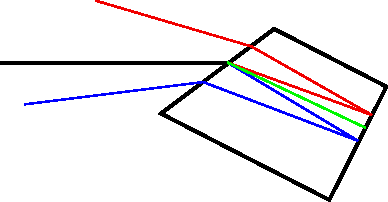
\includegraphics[width=.7\textwidth]{Littrow.pdf}
  \caption{Schematische Darstellung der Wellenlängenselektion mit einem Littrow- Prisma. Der grüne Strahl trifft senkrecht auf die reflektierende Rückseite des Prismas und wird zurück in den einfallenden schwarzen Strahl reflektiert.}
  \label{img:littrow}
\end{center}
\end{figure}



\subsection{Frequenzverdopplung}


Frequenzverdopplung oder auch Verdreifachung ist ein nichtlinearer Prozess von Licht in Materie.
Durchläuft Licht Materie, so werden die Elektronenhüllen aus ihrer Ruheposition ausgelenkt und fangen an zu schwingen. Für kleine Intensitäten ist diese Auslenkung näherungsweise harmonisch und
die schwingenden Dipole erzeugen wiederum Licht der gleichen Wellenlänge.
Wir die Intensität jedoch großer, so wird die Auslenkung stärker und die Elektronen wechselwirken zusätzlich mit Potentialen umliegender Kerne und die Auslenkung ist nicht mehr linear. 
Die führt zu dazu, dass im abgestrahlten Licht der Dipole auch die höheren Harmonischen enthalten
sind. Dieser Prozess ist zum einen Stark von der Intensität des einfallenden Lichts, aber auch
vom Material abhängig. Die Terme höherer Ordnung der dielektrischen Suszeptibilität eines Materials, welche in der Regel deutlich kleiner als der lineare Term sind, bestimmen die Effektivität der Generierung Frequenzvervielfachter Strahlung.




\subsection{Laserschutzbrillen}

\begin{figure}[H]
\begin{center}
  \includegraphics[width=.7\textwidth]{Schutzbrillen.png}
  \caption{Absorptions- (blau)  und Transmissionsspektrum (rot) der im Versuch
  verwendeten Laserschutzbrillen \cite{Versuchsanleitung}.}
  \label{img:Schutzbrillen}
\end{center}
\end{figure}

Abb.~\ref{img:Schutzbrillen} zeigt das Absorptions- und Transmissionsspektrum der
Laserschutzbrillen, die im Versuch verwendet werden.
Strahlung mit Wellenlängen unter 450\,nm wird um einem Faktor von mehr als $10^6$ abgeschwächt und
der starke blaue Pumplaser bei 444\,nm damit fast vollständig blockiert.
Bei Wellenlängen über 500\,nm beginnt eine signifikante Transparenz und über 550\,nm gelangt mehr
als 90\,\% des Lichts durch die Schutzbrillen,
so dass die Linien des Pr:YLF-Lasers beobachtet werden können.

